\chapter{Practice: Sleep}
Flash an XBee with the End-Device AT firmware using X-CTU.
First, plug the XBee in the XBee explorer socket and connect the USB cable.
Use the \texttt{dmesg} command to find to which device is the USB attached.
Look for a line similar to

\texttt{[ 6370.421000] usb 3-2.2: FTDI USB Serial Device converter now attached to ttyUSB0}

The command to invoke X-CTU will be something similar to

\texttt{wine .wine/drive\_c/Program{\textbackslash} Files/Digi/XCTU/X-CTU.exe}

Then set the port as in Fig. \ref{fig:set-port} and test that you can connect to the XBee using the ``Test/Query'' button as in Fig.~\ref{fig:test-xctu}.
\begin{figure}[htbp]
  \centering
  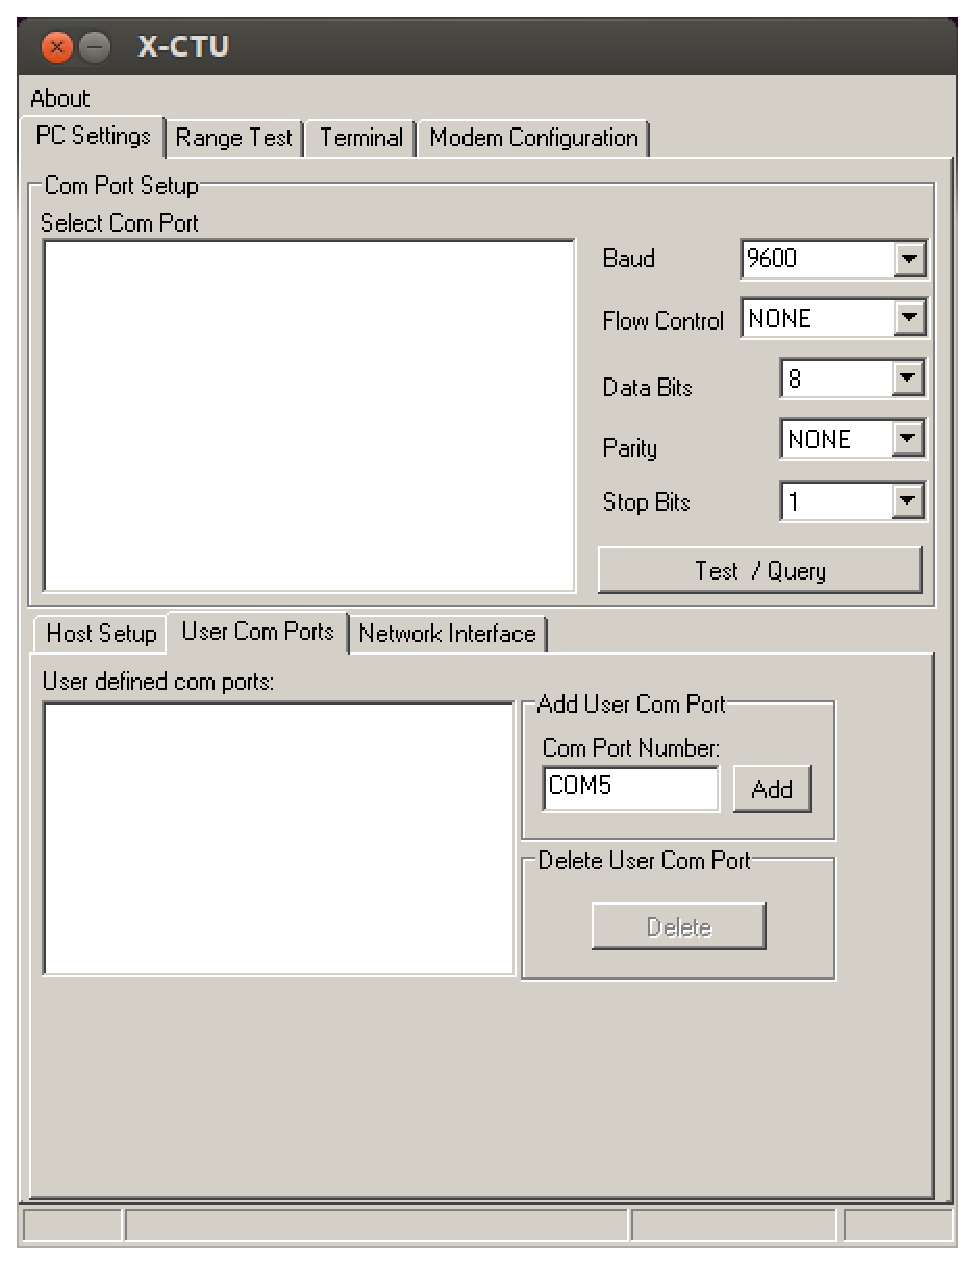
\includegraphics[width=0.3\linewidth]{figures/set-port.eps}
  \caption{Setting the port.}
  \label{fig:set-port}
\end{figure}

\begin{figure}[htbp]
  \centering
  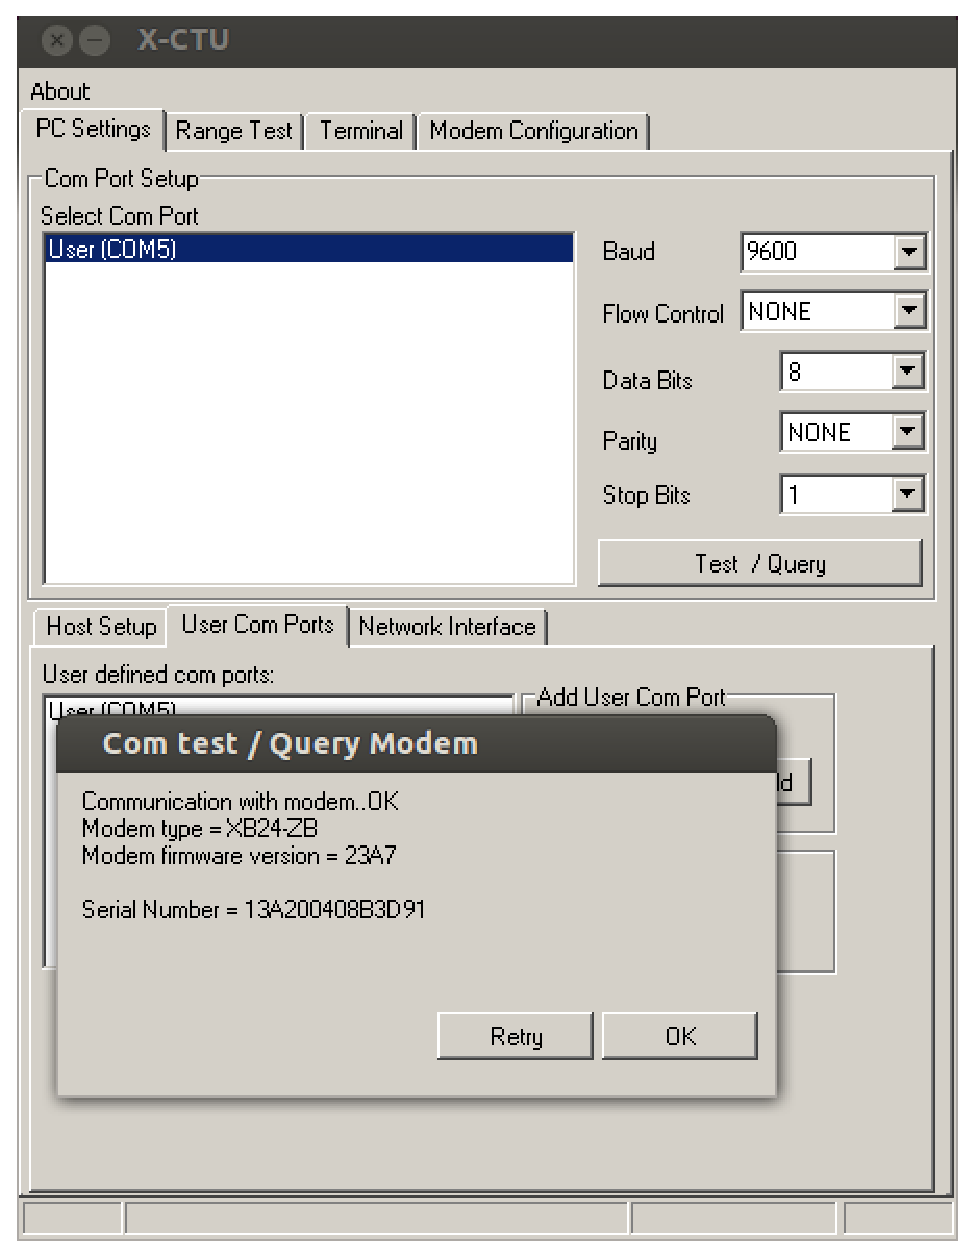
\includegraphics[width=0.3\linewidth]{figures/test-xctu.eps}
  \caption{Testing communication with the XBee.}
  \label{fig:test-xctu}
\end{figure}

Now we switch to the ``Modem Configuration'' tag.
We will flash the XBee with an ``end device'' firmware.
Only end devices can sleep.
Routers and coordinators must be always up.
We choose, for example, the firmware ``zigbee end device at'' in the ``Function set'' drop down menu.
And we write the firmware to the XBee.

Let's also clean all previous configuration.
Click the ``restore'' and ``read'' buttons to restore settings to defaults.
You should obtain something similar to Fig. \ref{fig:clean-28a7}.

\begin{figure}[htbp]
  \centering
  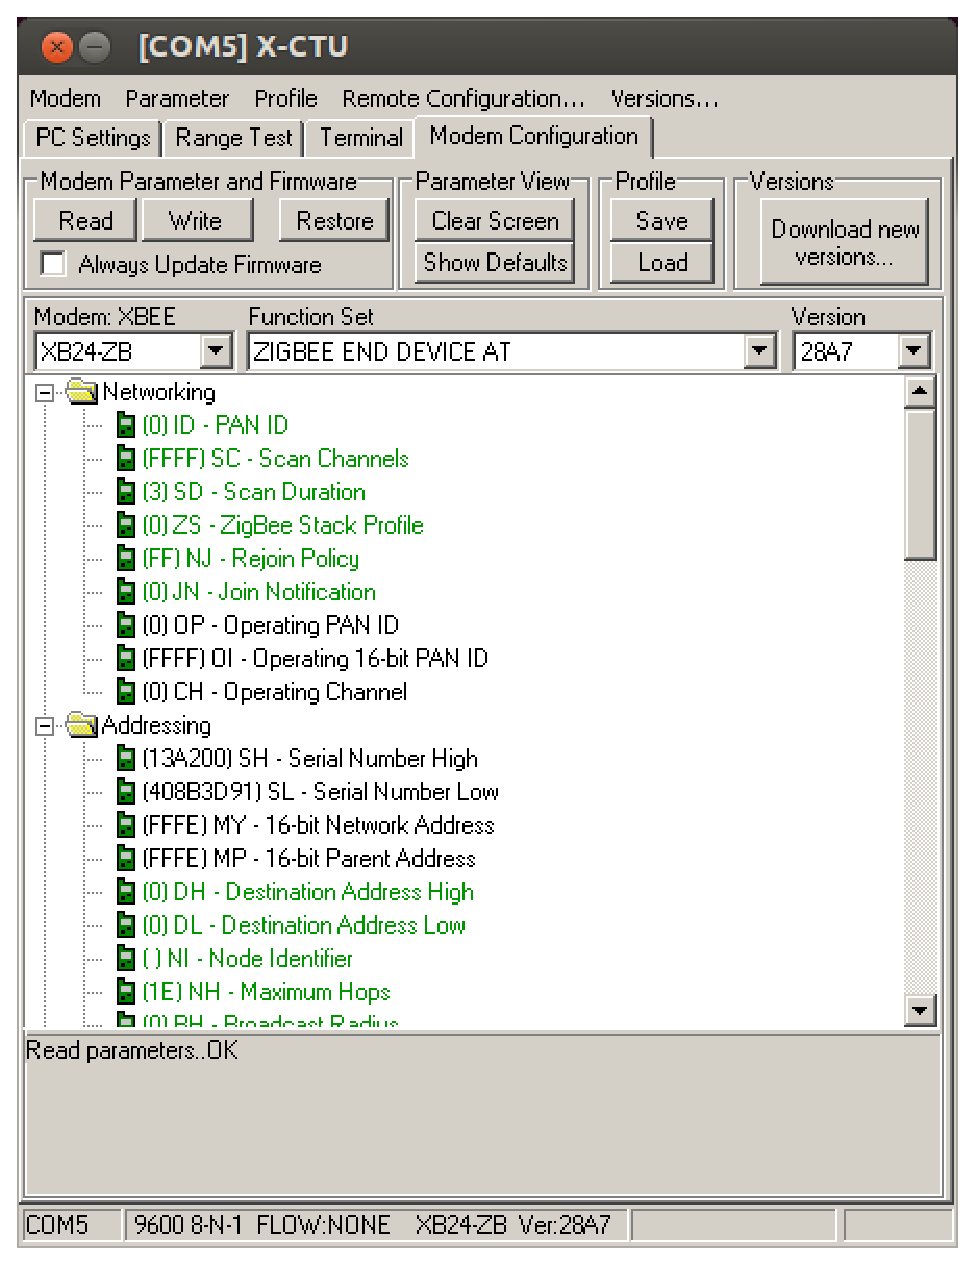
\includegraphics[width=0.3\linewidth]{figures/clean-28a7}
  \caption{Clean 28a7}
  \label{fig:clean-28a7}
\end{figure}

Let's prepare the new configuration.
Set the PAN ID to your group ID.
Set D0 to analog (2).
Set the sampling rate to 255 ms (IR=FF).
We write the changes to the XBee.
The configuration should look as shown in Fig. \ref{fig:configured-end-device}

\begin{figure}[htbp]
  \centering
  \includegraphics[width=0.3\linewidth]{figures/configured-end-device}
  \caption{Configured end device. D0 set to 2 and IR set to FF.}
  \label{fig:configured-end-device}
\end{figure}

Now we need to configure the coordinator just as we configured it for 
Chapter \ref{cha:sink-in-server}.
We write a coordinator API firmware and restore to factory defaults.

We set the PAN ID.
We set the AP to 2.
And we write the configuration.

Now run the python program to read incoming data, and we will see as our screens fills with the received data, as in Fig. \ref{fig:received-data}.

\begin{figure}[htbp]
  \centering
  \includegraphics[width=0.3\linewidth]{figures/received-data}
  \caption{Data received by the XBee connected to the computer.}
  \label{fig:received-data}
\end{figure}


Repeat the lab assignment ``collecting data in a computer'' but this time the sensors will be awake for 1 second and then sleep for 10 seconds.
While the sensor is awake, it will send a sample every 100ms.

